
\begin{figure}[h!]
\centering

    \begin{subfigure}[t]{0.48\textwidth}
    \centering
        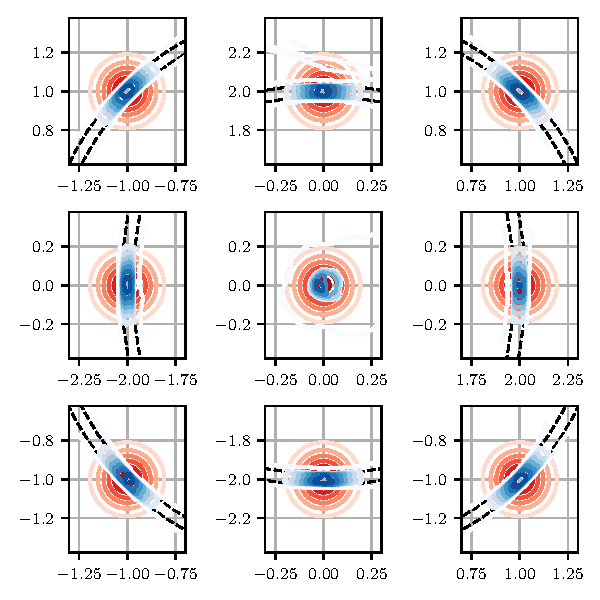
\includegraphics[width=0.95\textwidth]{figures/RNF_cluster_2019_09_26_12_27_27/RNF_density_array_1balls_00_00000_line.pdf}
        \vspace*{-0.2cm}
        \caption{}
        \label{fig:ring:space}
    \end{subfigure}%

    \begin{subfigure}[t]{0.24\textwidth}
        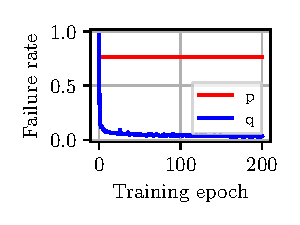
\includegraphics[width=\textwidth]{figures/RNF_cluster_2019_09_26_12_27_27/nf_bot_rate.pdf}
        \vspace*{-0.7cm}
        \caption{}
        \label{fig:ring:ar}
    \end{subfigure}%
    ~%
    \begin{subfigure}[t]{0.24\textwidth}
        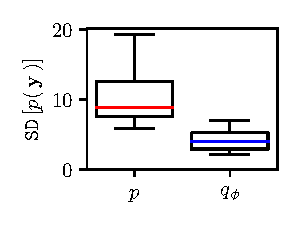
\includegraphics[width=\textwidth]{figures/RNF_cluster_2019_09_26_12_27_27/smc_variance_plot.pdf}
        \vspace*{-0.7cm}
        \caption{}
        \label{fig:ring:smc:var}
    \end{subfigure}
\vspace*{-0.2cm}
\caption{Results for the annulus problem introduced in Section \ref{sec:annulus}, where the acceptable region of perturbations is inside the black dashed band.
\ref{fig:ring:space} shows in blue the learned state-dependent proposal distribution over velocity (for a state at rest) is the well-approximating the original proposal (shown in red) \emph{inside} the acceptable region, with minimal mall in the invalid region, all but eliminating rejection as shown in \ref{fig:ring:ar}.
\ref{fig:ring:smc:var} shows the reduction in the variance of the evidence by using $q_{\phi}$.
We compute the variance using $100$ independent SMC sweeps, each using $100$ particles, and compare across $100$ datasets.
}
\label{fig:ring}
\end{figure}
